%%%%%%%%%%%%%%%%%%%%%%%%%%%%%%%%%%%%%%%%%%%%%%%%%%%%%%%%%%%%%%%%%%%%%%%%%%%%%%%%
% CS 2640 Final Report — Erasure Codes for Distributed Storage
%%%%%%%%%%%%%%%%%%%%%%%%%%%%%%%%%%%%%%%%%%%%%%%%%%%%%%%%%%%%%%%%%%%%%%%%%%%%%%%%

\documentclass[letterpaper,twocolumn,10pt]{article}
\usepackage{usenix2019_v3}

\usepackage{tikz}
\usepackage{amsmath}
\usepackage{graphicx}
\usepackage{booktabs}

\graphicspath{{imgs/}}

%-------------------------------------------------------------------------------
\begin{document}
%-------------------------------------------------------------------------------

\date{}

\title{\Large \bf Erasure Codes for Distributed Storage:\\
  Implementation and Trace-Driven Evaluation}

\author{
{\rm Xuanlin Jiang}\\
Harvard University \quad CS 2640
}

\maketitle

%-------------------------------------------------------------------------------
\begin{abstract}
%-------------------------------------------------------------------------------
Erasure codes promise fault tolerance with less storage than replication, but
their I/O latency under realistic workloads --- particularly while a disk is
out --- is poorly characterised. The gap is sharpest for
\emph{regenerating} codes (MSR, MBR): despite over a decade of theoretical
work establishing their optimality on the storage--repair-bandwidth tradeoff,
no mainstream erasure-coding library ships them, and the academic literature
on them is dominated by code constructions and information-theoretic bounds
rather than empirical benchmarks against the RAID/RS family they aim to
displace. I implement four representative codes (RAID-10, Reed--Solomon,
MSR, MBR) under a single C++17 interface and drive them with a trace-replay
discrete-event simulator over Microsoft Research Cambridge block I/O traces,
yielding a side-by-side comparison on the same workload, simulator and
failure scenario. The central abstraction is a \emph{DiskRequest
DAG} with \texttt{on\_ready} closures, which lets each code express
read--compute--write dependencies (parity deltas, regenerating-code repair
matrices) without coupling its math to the simulator. I reproduce the
textbook storage--repair tradeoff at fixed $(n,k)$ and find that the
degraded-mode latency penalty of regenerating codes is a fixed
$\alpha$-symbol cost that amortises with dataset size: at $100\times$ scale,
MSR's read-latency penalty drops from $1.77\times$ to $1.01\times$. At cloud
scales, MSR's small-storage advantage over MBR is therefore essentially free
in latency.
\end{abstract}

%-------------------------------------------------------------------------------
\section{Introduction}
\label{sec:intro}
%-------------------------------------------------------------------------------

Production storage systems at exabyte scale cannot afford full replication:
the storage tax is too high, and large clusters see daily disk failures.
Facebook's HDFS-RAID deployment, for example, replaced 3-way replication
with a $(10,4)$ Reed--Solomon code to recover petabytes of capacity, and
then a custom locally-repairable code to cut the resulting repair
traffic~\cite{sathiamoorthy13}.
Erasure codes, from RAID-6 and Reed--Solomon to recent
\emph{regenerating} codes such as MSR and MBR~\cite{dimakis10,rashmi11},
trade replication for parity computation. They promise the same fault
tolerance as multi-way replication using only a fraction of the storage,
and --- in the case of regenerating codes --- a fraction of the
repair-network bandwidth as well.

Yet the regenerating-code half of this design space is almost untouched in
practice. Mainstream production-grade erasure-coding libraries ---
Jerasure, Intel ISA-L, HDFS-EC, Ceph --- ship Reed--Solomon and
locally-repairable variants, but none ships an MSR or MBR implementation.
The academic literature mirrors that gap: existing work on regenerating
codes is overwhelmingly construction- and bound-oriented, with very little
side-by-side empirical comparison against the RAID/RS family that operators
actually deploy. A practitioner deciding whether the storage savings of MSR
or the repair-bandwidth savings of MBR are worth the engineering cost has
essentially no measured answer to fall back on.

What is much less well understood, then, is what these codes look like under
\emph{live load} and how they sit relative to the mature RAID/RS family.
Most prior work compares codes analytically or with microbenchmarks. The
question I set out to answer is concrete: when a disk fails and the system
must serve foreground I/O in degraded mode, which code wins on tail
latency, where do the regenerating codes actually land in the
storage--bandwidth--latency tradeoff space against RAID and RS, and how
does all of that change as the workload, the dataset, or the failure
scenario varies?

This paper makes three contributions. \textbf{(1)} A unified C++ implementation
of seven codes (RAID-0, RAID-1, RAID-6, RAID-10, RS, MSR, MBR) sharing one
abstract interface --- including from-scratch MSR and MBR implementations,
which to my knowledge are not provided by any production-grade erasure-coding
library --- with the four most representative evaluated end-to-end on the
same workload, simulator and failure scenario. \textbf{(2)} A trace-driven
discrete-event simulator built around a \texttt{DiskRequest} DAG
abstraction whose \texttt{on\_ready} closures let each code express its
GF($2^8$) compute inline with its I/O dependencies, without leaking coding
logic into the simulator. \textbf{(3)} An empirical placement of MSR and
MBR in the storage--bandwidth--latency tradeoff space alongside the mature
RAID/RS codes, including the headline finding that the regenerating-code
degraded-mode penalty is a fixed $\alpha$-symbol cost that \emph{amortises}
as the dataset grows: at $100\times$ scale MSR's penalty all but disappears. The rest of the paper
covers background and the threat model (\S\ref{sec:bg}), system design
(\S\ref{sec:design}), implementation details (\S\ref{sec:impl}),
experiments (\S\ref{sec:exp}), discussion (\S\ref{sec:disc}), and
conclusion (\S\ref{sec:conc}).

%-------------------------------------------------------------------------------
\section{Background and Motivation}
\label{sec:bg}
%-------------------------------------------------------------------------------

\paragraph{Erasure codes.}
An $(n,k)$ erasure code maps $k$ data symbols onto $n$ stored symbols on $n$
distinct nodes. A code is \emph{maximum-distance-separable} (MDS) if any $k$
of the $n$ nodes suffice to reconstruct the original data; classical
Reed--Solomon~\cite{reed60,plank97} and RAID-6 are MDS. \emph{Regenerating}
codes~\cite{dimakis10} relax the per-node read pattern: instead of pulling
$k$ entire nodes during repair, a new node contacts $d$ \emph{helper} nodes
and downloads only $\beta$ symbols from each, for a total repair traffic of
$d\beta$. Each node stores $\alpha$ symbols per stripe.

\paragraph{The storage--repair tradeoff at fixed $(n,k)$.}
For fixed $(n,k,d)$, $(\alpha,\beta)$ trace out a curve. Two endpoints are
of practical interest: the \emph{minimum-storage regenerating} (MSR) point
minimises $\alpha = d-k+1$, and the \emph{minimum-bandwidth regenerating}
(MBR) point minimises $d\beta$ at the cost of $\alpha = d$. For
$(n,k,d)=(6,3,5)$ this gives MSR $\alpha=3$ and MBR $\alpha=5$. The two
families are summarised below:

\begin{center}
\small
\begin{tabular}{@{}lccl@{}}
\toprule
Family & Storage & Repair BW & Examples \\
\midrule
MDS & optimal & $k$ symbols & RS, RAID-6 \\
Regenerating & near-opt. & $d\beta$ symbols & MSR, MBR \\
\bottomrule
\end{tabular}
\end{center}

\paragraph{Reliability is a separate axis.}
The four codes I evaluate --- RAID-10$(6,3)$, RS$(6,3)$, MSR$(6,3,5)$ and
MBR$(6,3,5)$ --- have \emph{non-identical} reliability profiles even at the
same $(n,k)$. RS, MSR and MBR all tolerate any $n-k=3$ disk failures.
RAID-10$(6,3)$, in contrast, tolerates 3 simultaneous failures only if no
two of them are mirrored siblings; otherwise the array loses data. The four
points therefore lie in a tradeoff \emph{space}, not on a single Pareto
frontier; reliability is held only partially fixed by the parameter choice.
I return to this caveat when discussing the storage--repair plot in
\S\ref{sec:exp}.

\paragraph{The implementation and evaluation gap.}
Reed--Solomon and RAID-6 are mature: production libraries (Jerasure,
Intel ISA-L, HDFS-EC, Ceph) ship them, and decades of deployment
experience characterise their behaviour. Regenerating codes are not.
None of the mainstream libraries above ships an MSR or MBR
implementation, and the published literature on these codes
remains weighted toward existence proofs, capacity bounds, and code
constructions rather than empirical comparisons against the RAID/RS
family they aim to displace. The result is a design space with one
half mapped in detail and the other half mapped only on paper. This
project contributes implementations of MSR and MBR alongside RAID-10
and RS under one interface specifically so the two halves can be
compared head-to-head.

\paragraph{Why latency under load is the right question.}
Real workloads are skewed in size, op-mix, and arrival distribution. Public
Microsoft Research Cambridge (MSRC) block I/O
traces~\cite{narayanan08} from production servers see request sizes from
$0.5$~KB to $250$~KB and read/write ratios that vary by an order of
magnitude across volumes. Closed-form analyses of repair bandwidth do not
predict how a code will saturate, what its tail latency looks like in
degraded mode, or how either changes with dataset size --- exactly the
questions a deployment must answer.

\paragraph{Threat model.}
Steady-state replay of a real workload, single permanent disk failure
mid-trace, foreground I/O continues in degraded mode. I do \emph{not}
overlap repair traffic with foreground I/O in the timing experiments;
repair correctness is verified separately. Multi-failure and
repair-under-load are future work (\S\ref{sec:disc}).

%-------------------------------------------------------------------------------
\section{Design}
\label{sec:design}
%-------------------------------------------------------------------------------

The system is two layers (Fig.~\ref{fig:arch}). A \textbf{codes library}
implements each erasure code behind one abstract \texttt{ErasureCode}
interface; a \textbf{simulator library} replays traces against either an
in-memory \texttt{StorageArray} (for correctness verification) or a
discrete-event simulator \texttt{DESSimulator} (for timing). The two layers
communicate through a single data structure --- the \texttt{DiskRequest} ---
that carries enough metadata to express read--compute--write dependencies
without ever coupling coding math to scheduling.

\begin{figure}[t]
  \centering\small
  \begin{tabular}{|c|}
  \hline
  \texttt{sim\_main} \quad / \quad test suite \\
  \hline
  \texttt{DESSimulator} \quad \texttt{StorageArray} \\
  \texttt{TraceTranslator} \\
  \hline
  RAID-0/1/6/10, RS, MSR, MBR \\
  \texttt{gf256}, \texttt{matrix\_gf256} \\
  \hline
  \end{tabular}
  \caption{Two-layer architecture. The codes library has no dependency on
  the simulator; both executors consume the same \texttt{DiskRequest} DAG.}
  \label{fig:arch}
\end{figure}

\paragraph{The \texttt{ErasureCode} interface.} Three calls dominate:
\texttt{translate(lb,nb,rw,data,bs)} converts a logical I/O into a vector of
\texttt{DiskRequest}s; \texttt{assembleRead(...)} reassembles logical data
from the filled read requests; and \texttt{repair(disk\_cap,bs)} returns the
DAG that rebuilds a failed disk. The same calls drive both modes:
\texttt{block\_size = 0} means \emph{sim mode} (no data movement,
timing-only), $>0$ means \emph{verify mode} (data buffers carried). Codes
generate requests; they never touch storage.

\paragraph{The \texttt{DiskRequest} DAG.} This is the system's central
abstraction. Each request carries an \texttt{id}, a \texttt{depends\_on}
list of local IDs that must complete first, an optional shared buffer
\texttt{buf}, and an optional \texttt{on\_ready} closure invoked just before
the request is issued. The closure's job is to do the GF($2^8$) work that
sits \emph{between} the dependent reads and the dependent write --- for
example, in a parity update: read old data and old parity, XOR-and-multiply
to compute the new parity, then write it. Without \texttt{on\_ready}, the
simulator would have to know about parity arithmetic; with it, the
simulator only walks the DAG. The verifier executes the DAG via Kahn's
topological sort; the simulator decrements per-request \texttt{dep\_count}s
on each \texttt{DiskCompletion} event and enqueues newly-ready requests.

\paragraph{Two-phase experiment timeline.}
Each experiment replays the trace twice against an isolated array: once
with no failure (\emph{normal} phase, baseline) and once with a designated
disk marked failed before replay starts (\emph{degraded} phase). The two
phases share their seeded arrival sequence so latency differences come
purely from the code's degraded-mode I/O pattern. Repair latency is not
measured under load; the repair DAG is exercised separately for correctness
(\S\ref{sec:impl}).

%-------------------------------------------------------------------------------
\section{Implementation}
\label{sec:impl}
%-------------------------------------------------------------------------------

\paragraph{GF$(2^8)$ math.}
\texttt{gf256.\{h,cpp\}} provides $\log/\mathrm{antilog}$ tables for
addition (XOR), multiplication, inverse and exponentiation, all $O(1)$
table lookups. \texttt{matrix\_gf256.\{h,cpp\}} layers Gauss--Jordan inversion,
matrix multiply, and Cauchy/Vandermonde generators on top.

\paragraph{Per-code constructions.}
\textbf{RAID-0/1/10} are striping and mirroring (no GF math); only RAID-10
is exercised in the experiments. \textbf{RAID-6} computes a P (XOR) and a Q
($\sum_i \alpha^i x_i$) parity column over GF($2^8$); single-disk repair is
XOR, double-disk repair inverts a $2\times 2$ GF system. \textbf{RS$(n,k)$}
uses a systematic Cauchy generator; repair of $f \le n-k$ failed disks
inverts the corresponding $k\times k$ submatrix. \textbf{MSR$(n,k,d)$}
follows the layered RS construction with $\alpha = d{-}k{+}1$ symbols per
node. \textbf{MBR$(n,k,d)$} uses the Rashmi--Shah--Kumar product-matrix
construction~\cite{rashmi11} with $\alpha = d$. Each code lives in one
\texttt{.h}/\texttt{.cpp} pair under \texttt{src/codes/}.

\paragraph{Discrete-event simulator.}
\texttt{DESSimulator} is a priority queue keyed on event time. Events are
\texttt{RequestArrival}, \texttt{DiskCompletion}, and \texttt{DiskFailure}.
Each disk has its own FIFO queue; service time is deterministic
$\textit{size}/\textit{bandwidth}$. When a request lands, its
\texttt{dep\_count} (the number of unfinished prerequisites in its DAG) is
checked; if zero, \texttt{on\_ready} fires and the request is enqueued.
A \texttt{DiskCompletion} decrements every dependent's count and may
release new requests cascading through the DAG.

\paragraph{Trace translator.}
\texttt{TraceTranslator} reads pre-processed MSRC rows of the form
\texttt{(op, offset, size)}, discards the original timestamps, and
re-emits them as \emph{Poisson} arrivals at a configurable rate. This
decouples workload \emph{shape} (which I want to keep realistic) from
arrival \emph{rate} (which I sweep).

\paragraph{Verification by construction.}
Each code is exercised in a separate test (\texttt{test\_raid},
\texttt{test\_ec}) against an in-memory \texttt{StorageArray}: encode-then-decode
round-trip, single- and double-disk failure followed by \texttt{repair()},
read-back of the rebuilt disk, and partial-stripe (RMW) writes at unaligned
boundaries. The contract is byte-for-byte equality. All seven codes pass.
Repair latency is not part of the timing sweep in \S\ref{sec:exp}; this
section is where repair is exercised.

%-------------------------------------------------------------------------------
\section{Experiments}
\label{sec:exp}
%-------------------------------------------------------------------------------

\subsection{Setup}

\begin{center}
\small
\begin{tabular}{@{}ll@{}}
\toprule
Parameter & Value \\
\midrule
Disks $n$               & 6 \\
$(k, d)$                & $(3, 5)$ \\
Codes evaluated         & RAID-10, RS, MSR, MBR \\
Disk bandwidth          & 128 MB/s \\
Block / chunk           & 4 KB / 1 block \\
Trace                   & MSRC \texttt{mds\_1} (2007) \\
Requests per phase      & 10\,000 \\
Phases                  & normal, degraded \\
Arrivals                & Poisson, rate-swept \\
Failure                 & disk 0 (data); disk 3 (parity) for RS \\
RNG seed                & 42 \\
\bottomrule
\end{tabular}
\end{center}

\noindent I run two dataset sizes, \texttt{mds\_1} and \texttt{mds\_1\_100x}; the
latter scales the addressable dataset $100\times$ by spreading the same
trace across a proportionally larger logical address space, so that each
stripe is touched by many more logical I/Os.

\subsection{The storage--repair tradeoff}

Figure~\ref{fig:tradeoff-A} plots the four codes in the
(repair-download, total-storage) plane, normalised to RAID-10. The MSR and
MBR points sit on the analytic MSR$\leftrightarrow$MBR boundary curve;
RS lies far to the right (it pays $k$ symbols of repair traffic per failed
symbol); RAID-10 sits at $(1,1)$ by construction. As cautioned in
\S\ref{sec:bg}, the four points are \emph{not} comparable as a strict Pareto
frontier: RAID-10 trades reliability for those low coordinates.

\begin{figure}[t]
  \centering
  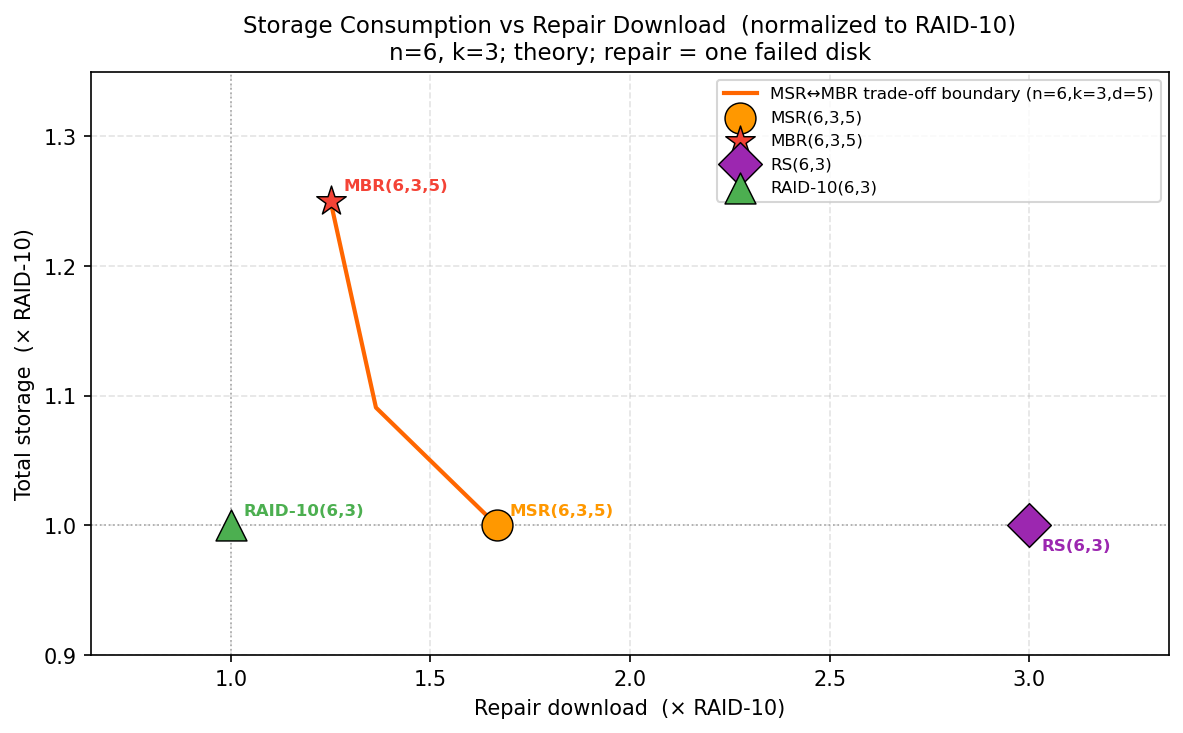
\includegraphics[width=\columnwidth]{mds_1/tradeoffs_A_repair_storage.png}
  \caption{Storage vs.\ repair download, normalised to RAID-10. The four
  evaluated codes do \emph{not} share the same reliability guarantee:
  RAID-10$(6,3)$ tolerates 3 failures only if no siblings fail, whereas
  RS/MSR/MBR tolerate any 3.}
  \label{fig:tradeoff-A}
\end{figure}

\subsection{Load--latency: normal vs.\ degraded}

Figure~\ref{fig:load-latency} sweeps Poisson arrival rate against average
latency for both dataset sizes. At low load all codes converge near the
disk service time. As load rises the curves bend upward at different
points; the saturation knee is where the response cliff begins.

\textbf{$1\times$ dataset (Fig.~\ref{fig:load-latency}, left):} the
saturation order is $\mathrm{MBR} < \mathrm{MSR} < \mathrm{RS} <
\mathrm{RAID\text{-}10}$. MBR saturates first because its $\alpha = d = 5$
makes every logical I/O fan out to many disk requests; RAID-10 saturates
last because each I/O hits at most a single stripe replica.

\textbf{$100\times$ dataset (Fig.~\ref{fig:load-latency}, right):} the order
becomes $\mathrm{MBR} < \mathrm{MSR} \approx \mathrm{RS} \approx
\mathrm{RAID\text{-}10}$. MSR closes the gap to the MDS codes once its
$\alpha$ cost is amortised across many more logical I/Os per stripe; MBR
still trails because its $\alpha$ is larger.

In both panels the degraded curves (dashed) peel away from the normal
curves (solid) at mid-load; the gap is much smaller at $100\times$.

\begin{figure*}[!t]
  \centering
  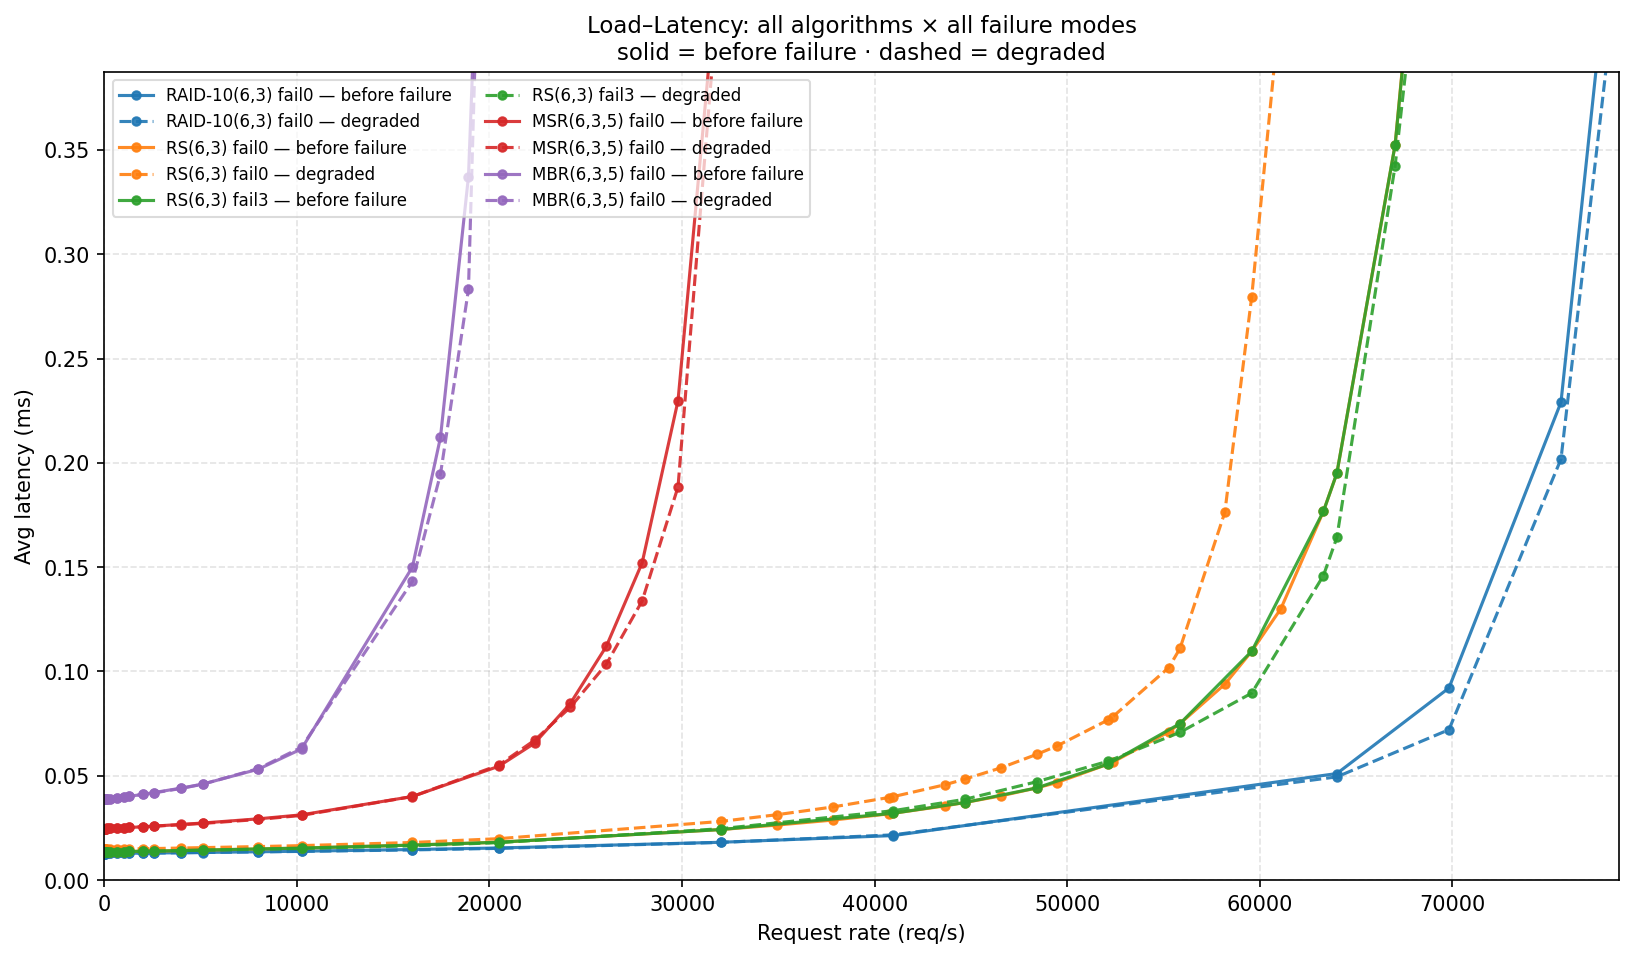
\includegraphics[width=0.49\textwidth]{mds_1/load_latency.png}\hfill
  
\includegraphics[width=0.49\textwidth]{mds_1_100x/load_latency.png}
  \caption{Load--latency at $1\times$ (left) and $100\times$ (right) dataset
  scale. Solid lines are normal phase, dashed lines are degraded.
  Saturation order at $1\times$:
  $\mathrm{MBR}<\mathrm{MSR}<\mathrm{RS}<\mathrm{RAID\text{-}10}$;
  at $100\times$ the gap between MSR and the MDS codes closes.}
  \label{fig:load-latency}
\end{figure*}

\begin{figure*}[!htbp]
  \centering
  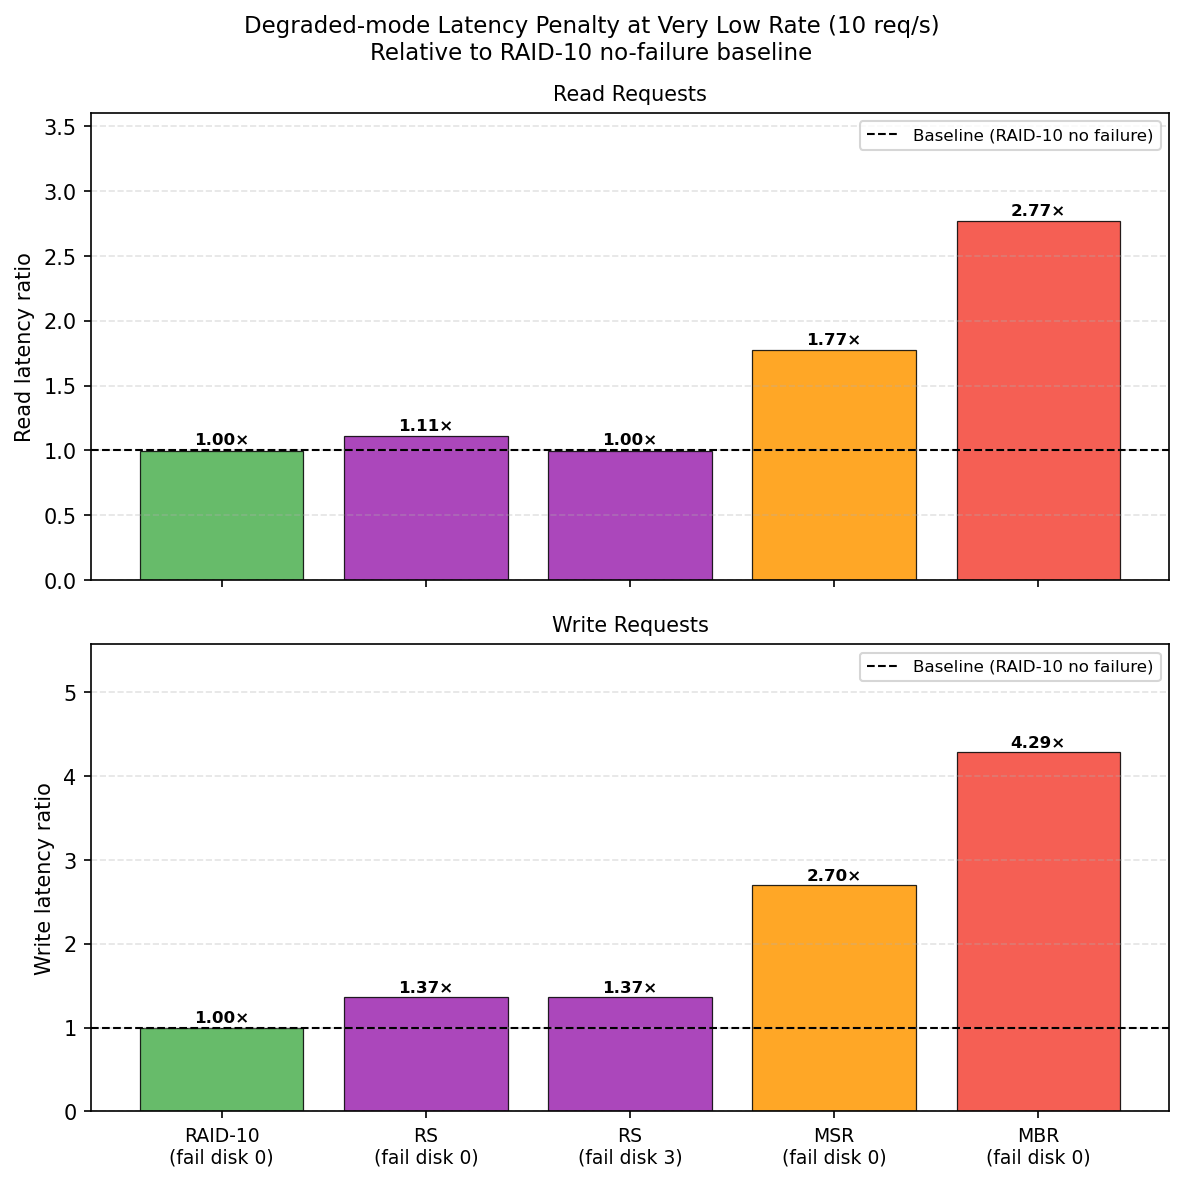
\includegraphics[width=0.42\textwidth]{mds_1/tradeoffs_B_latency_penalty.png}\hfill
  
\includegraphics[width=0.42\textwidth]{mds_1_100x/tradeoffs_B_latency_penalty.png}
  \caption{Degraded-mode latency penalty (relative to RAID-10 no-failure
  baseline) at $1\times$ scale (left) and $100\times$ scale (right).
  At $100\times$ MSR drops to $1.01\times$ on reads; the regenerating-code
  penalty amortises with dataset size.}
  \label{fig:tradeoff-B}
\end{figure*}

\subsection{Degraded-mode latency penalty}

Figure~\ref{fig:tradeoff-B} reports the ratio of degraded-phase to baseline
latency at very low load (so queueing effects do not mask the coding cost).
At $1\times$, regenerating codes pay heavily: MSR's read penalty is
$1.77\times$, MBR's $2.77\times$, while RS adds only $1.11\times$ on a data
disk and effectively zero on a parity disk; RAID-10 is at the baseline.
Writes show the same ordering and amplified ratios (RAID-10 $1.00\times$,
RS $1.37\times$, MSR $2.70\times$, MBR $4.29\times$) because each write
touches more stripes worth of repair work.

\subsection{Effect of dataset size: $\alpha$ amortisation}

The $100\times$ panel of Fig.~\ref{fig:tradeoff-B} is the headline result.
At cloud-storage scale the regenerating-code penalty all but vanishes:
MSR's read penalty drops from $1.77\times$ to $1.01\times$ and its write
penalty from $2.70\times$ to $1.03\times$. MBR's penalty also shrinks
($2.77\times \to 1.26\times$ on reads, $4.29\times \to 1.29\times$ on
writes), but it is asymptotically larger because $\alpha = d$ is bigger.
The reason is structural (\S\ref{sec:disc}): each repair pays a fixed cost
\emph{per $\alpha$-symbol stripe}, and a $100\times$ dataset spreads that
fixed cost across $100\times$ as many logical I/Os.

%-------------------------------------------------------------------------------
\section{Discussion}
\label{sec:disc}
%-------------------------------------------------------------------------------

\paragraph{Why $\alpha$-amortisation works.}
Repair (and degraded-mode reads, which structurally resemble repair) pays a
fixed cost per $\alpha$-symbol stripe: read $\alpha$ surviving symbols, do
GF($2^8$) work, write $\alpha$ recovered symbols. That cost is independent
of how many logical I/Os hit the stripe. Larger datasets dilute it across
more I/Os, so the per-request penalty falls.

\paragraph{Practical implication.}
At cloud scale the storage cost \emph{dominates} the choice between MSR and
MBR: MBR pays $1.25\times$ more storage for an asymptotic latency
disadvantage. MSR's $1\%$ read penalty at $100\times$ is essentially free
relative to its storage savings.

\paragraph{Limitations.}
I model a single permanent failure; multi-failure correlated scenarios are
not exercised. Disk service time is deterministic, ignoring internal
queueing in real devices. GF($2^8$) compute time is treated as
instantaneous, which understates CPU-bound codes. Most importantly, repair
traffic is not overlapped with foreground I/O in the latency sweep --- a
real system would have to amortise the $\alpha$-cost \emph{plus} the cost of
the rebuild itself.

%-------------------------------------------------------------------------------
\section{Conclusion}
\label{sec:conc}
%-------------------------------------------------------------------------------

I implemented four representative erasure codes --- including from-scratch
MSR and MBR, which are absent from production erasure-coding libraries ---
under one abstract interface and drove them with a trace-replay DES whose
central \texttt{DiskRequest}-DAG abstraction lets each code express its
GF($2^8$) work as closures attached to its I/O dependencies. Putting the
regenerating codes side-by-side with the mature RAID/RS family on the
same workload places them concretely in the
storage--bandwidth--latency tradeoff space rather than only on paper:
the textbook storage--repair tradeoff at fixed $(n,k)$ holds in my
measurements, and the regenerating-code degraded-mode penalty amortises
with dataset size to $\sim 1\%$ for MSR at $100\times$ scale --- a
practical answer to the question of whether MSR is deployable that the
prior literature did not provide. Future work: multi-failure
scenarios, repair traffic concurrent with foreground I/O, GF($2^8$)
compute-time accounting, and lazy-vs-eager repair scheduling.

%-------------------------------------------------------------------------------
\bibliographystyle{plain}
\bibliography{report}

\end{document}
